\begin{figure}[H]
    \centering
    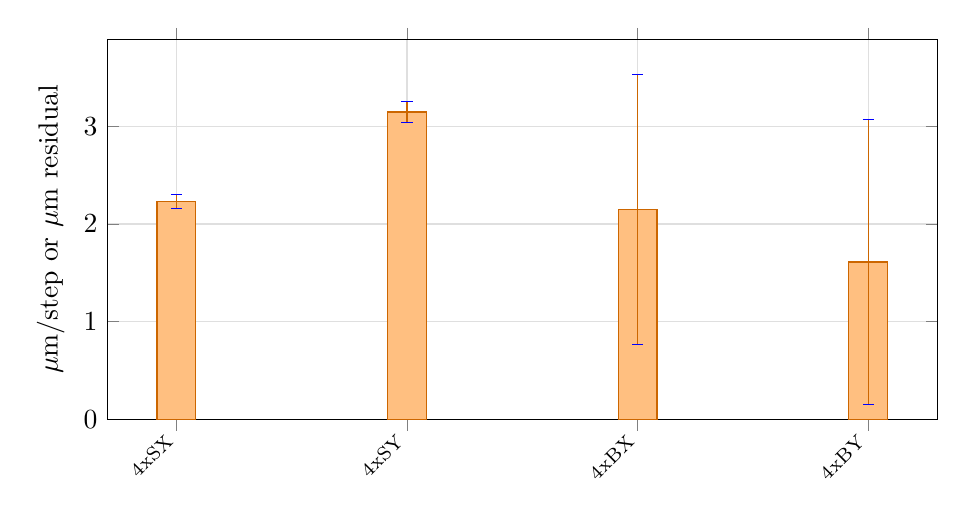
\begin{tikzpicture}
        \begin{axis}[
            width=\linewidth,
            height=6.4cm,
            ybar,
            bar width=14pt,
            ymin=0,
            ylabel={$\mu$m/step or $\mu$m residual},
            symbolic x coords={4xSX,4xSY,4xBX,4xBY},
            xtick=data,
            xticklabels={4xSX,4xSY,4xBX,4xBY},
            x tick label style={rotate=45, anchor=east, font=\scriptsize},
            error bars/y dir=both, error bars/y explicit,
            grid=major,
            major grid style={draw=gray!25},
        ]
        \addplot+[fill=orange!50, draw=orange!80!black] coordinates {
(4xSX,2.2319) +- (0,0.0699)
(4xSY,3.1475) +- (0,0.1098)
(4xBX,2.1503) +- (0,1.3846)
(4xBY,1.6109) +- (0,1.4640)
        };
        \end{axis}
    \end{tikzpicture}
    \caption[4x calibration-repeatability results]{Calibration-repeatability results for the 4x objective profile. SX/SY are repeated stage-scale estimates. BX/BY are residual displacements after backlash reversal checks. Error bars show one standard deviation.}
    \label{fig:eval-calibration}
\end{figure}
